\section{Experimental Setup and Results}
\label{sec:exp}

\paragraph{Data and training.}
Models train on about 225\,h: 77\,h of English read speech (a LibriSpeech~\cite{panayotov2015librispeech} subset), 108\,h of Nepali (internally prepared studio recordings and read speech, including OpenSLR Nepali), and 34\,h of code-mixed speech. Utterances are 1--12\,s, and sentences in validation or test splits are removed from training. For a single cross-lingual target voice, a fine-tuned OmniVoice~\cite{omnivoice2026} teacher synthesized English and Nepali in one voice (22.7\,h EN, 15.7\,h NE), kept only when an independent ASR transcribed it with CER $\le$0.10 (EN) or $\le$0.12 (NE). Supplementary synthetic Nepali receives half the loss weight of human recordings. Training is multi-speaker (1,815 speakers); exported models keep one speaker vector. Training runs in BF16 on one RTX~4090 with L1 log-mel, multi-resolution STFT, duration, $F_0$/voicing and energy losses plus multi-period/multi-resolution adversarial and feature-matching losses. On half of the steps the acoustic network is conditioned on its own predicted prosody rather than ground truth, which closed a large train/inference gap. Durations come from Viterbi forced alignment with a training-only CTC phoneme recognizer~\cite{graves2006ctc}.

\subsection{Clean \texttt{v3} Data Alignment (\texttt{EXP-014})}
Early training (\texttt{v2}) predated the final Nepali lexicon and \textit{va} $\rightarrow$ \texttt{/b/} rule update. Rebuilding the 136,807-utterance feature cache (\texttt{v3}) with the current frontend, retraining the frozen CTC phoneme recognizer (\texttt{ctc\_aligner\_v3.pt}, CTC loss $\approx$1.0 $\rightarrow$ 0.614), and re-extracting Viterbi forced-alignment durations reduced single-frame duration collapses by $\approx$3$\times$ and dropped spurious \textit{va}-word \texttt{/b/ $\rightarrow$ /w/} confusion on 300 Nepali test utterances from 55.1\% (65/118) to \textbf{0.0\%} (0/118). Fine-tuning on consistent labels then lowered validation PER from 7.06\% to 3.96\% (Nepali) and 5.29\% to 4.33\% (English; Figure~\ref{fig:labels}), measured on the in-training validation subset (Section~\ref{sec:wsp} uses a separate fixed 150+150 validation subset). This intervention is confounded: the labels, the recognizer, the durations and 10k additional training steps all changed together, with no continued-\texttt{v2} control. Because the recognizer that scores PER was retrained on the new labels, the 7.06\% and 3.96\% figures are not on a common scale; part of the drop reflects agreement with the new label conventions. The /b/$\to$/w/ result is a direct substitution count and is the more robust evidence.

\begin{figure}[t]
  \centering
  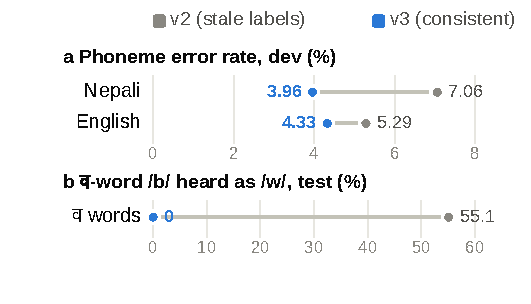
\includegraphics[width=\columnwidth]{figures/label_consistency.pdf}
  \caption{\textbf{Label consistency matters more than any edit.} Rebuilding the feature cache and phoneme recognizer with the current frontend (v2$\to$v3) nearly halves Nepali PER (a) and removes the spurious \textit{va}-word /b/$\to$/w/ errors that earlier looked like a model defect (b).}
  \label{fig:labels}
\end{figure}

\subsection{Bilingual Synthesis Quality and Equal-Budget 281K Ablation}
Table~\ref{tab:params} summarizes the parameter footprint and held-out evaluation across \texttt{PAWP-1.5M v3} (\texttt{EXP-015a}, 10k FT steps on \texttt{v3} from \texttt{EXP-012}) and the equal-budget 281K variants (\texttt{EXP-015b} Shared vs.\ \texttt{EXP-015c} Dense, trained from scratch for 36k steps on \texttt{v3}, identical recipe, \texttt{seed=42}). Held-out ASR is measured on $n=30$ EN, $n=30$ NE, and $n=9$ code-mixed utterances using a single recognizer (reported alongside the human studio audio floor as an intelligibility proxy, not a naturalness comparison). Untouched test PER is measured on $n=300$ NE + $n=300$ EN utterances via \texttt{ctc\_aligner\_v3.pt}, and minimal-pair contrast is scored acoustically on an internal 77-pair set (11 pairs in each of seven categories: four-way laryngeal, dental/retroflex, alveolar affricates, gemination, schwa deletion/flapping, sibilant merger/nasality, and English/code-mix contrasts). Both members of a pair are synthesized and decoded by the CTC recognizer. \emph{Distinct} is the fraction of pairs whose two decodings differ, and \emph{Exact} is the fraction where both decode exactly to their frontend phoneme strings.

\paragraph{Evaluation validity.}
Both automatic metrics have known circularity. (i)~PER is scored by \texttt{ctc\_aligner\_v3.pt}, the same recognizer that produced the training durations, trained on the same frontend labels. PER therefore measures consistency with the frontend's phoneme conventions, not absolute pronunciation correctness, and may miss distortions that stay inside the recognizer's decision boundaries. (ii)~The ASR service that scores held-out WER/CER is the same recognizer that filtered the synthetic target-voice corpus, which favours speech that this recognizer transcribes well. This explains why synthetic CER can fall below the human-recording floor (Figure~\ref{fig:asr}). Table~\ref{tab:indep} therefore re-scores all models with two recognizers that played no part in training or data filtering. Native-listener tests remain pending.

\paragraph{Independent re-scoring.}
Under independent recognizers (Table~\ref{tab:indep}), every synthetic system is \emph{worse} than the human recordings on English CER and on phone error rate in both languages, so the earlier below-human CER was a recognizer artifact. The independent ASR is weak on Nepali (human CER 22.65\%), and the phone recognizer was not trained on Nepali (human PER 34.12\%). Absolute Nepali numbers are therefore only coarse, and the comparisons below are paired on identical sentences. PAWP-1.5M remains close to the human reference on English (PER 15.14\% vs.\ 13.44\%; CER 2.35\% vs.\ 0.68\%). On a new 160-sentence code-mixed set (4.7 language switches per sentence, no textual overlap with training data, zero \texttt{<unk>} tokens), it reaches 18.13\% WER / 8.80\% CER (95\% CI 15.9--20.6\% WER), with more errors in English spans (21.9\%) than in Nepali spans (12.0\%). The phone recognizer also outputs no retroflex nasal on any of the 300 human Nepali utterances, so it can neither confirm nor refute the nasal finding of Section~\ref{sec:wsp}.

\begin{table*}[t]
\centering
\caption{End-to-end parameter footprint (all inference tensors counted) and evaluation on clean \texttt{v3} alignment. Held-out ASR uses a single recognizer ($n=30/30/9$, \texttt{seed=42}); untouched test PER uses \texttt{ctc\_aligner\_v3.pt} ($n=300$ NE + $300$ EN), reporting 3-seed mean $\pm$ std (\texttt{seeds 42, 101, 202}) for \texttt{EXP-015b/c}.}
\label{tab:params}
\footnotesize
\setlength{\tabcolsep}{4pt}
\resizebox{\textwidth}{!}{%
\begin{tabular}{@{}lrrrrrrr@{}}
\toprule
Model (\texttt{v3}) & Unique / Total & FP32 & EN ASR & NE ASR & Mix ASR & Test NE / EN & CTC 77-Pair \\
 & Params & Size & WER/CER & WER/CER & WER/CER & PER ($n=600$) & Distinct / Exact \\
\midrule
Human Floor (ASR) & --- & --- & 2.63 / 0.75 & 11.60 / 3.82 & 25.91 / 12.88 & --- & --- \\
\textbf{PAWP-1.5M v3} (\texttt{EXP-015a}) & 1,490,390 / 1,490,390 & 5.98\,MB & \textbf{4.02 / 1.50} & \textbf{12.35 / 1.75} & 12.32 / 5.32 & \textbf{5.04\% / 4.02\%} & \textbf{83.1\% / 58.4\%} \\
\textbf{PAWP-300K Shared} (\texttt{EXP-015b}) & 281,078 / 328,158 & 1.12\,MB & 6.88 / 2.93 & \textbf{19.71 / 5.93} & \textbf{12.02 / 5.01} & 6.35$\pm$0.11\% / 6.57$\pm$0.47\% & 77.9\% / 39.0\% \\
\textbf{Dense-300K} (\texttt{EXP-015c}) & 281,442 / 281,442 & 1.13\,MB & \textbf{6.15 / 2.42} & 20.21 / 6.59 & 18.09 / 9.01 & \textbf{5.53$\pm$0.08\% / 5.34$\pm$0.28\%} & 79.2\% / 37.7\% \\
\bottomrule
\end{tabular}}
\end{table*}

\begin{figure}[t]
  \centering
  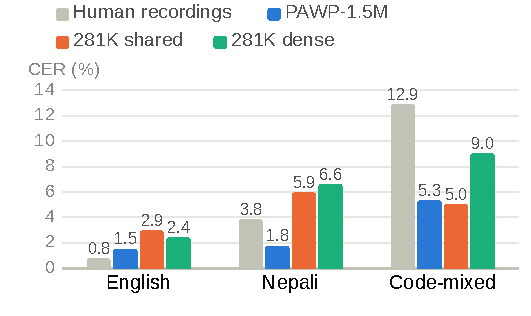
\includegraphics[width=\columnwidth]{figures/intelligibility.pdf}
  \caption{\textbf{Held-out ASR character error rate} (one recognizer; $n=30$ EN, 30 NE, 9 code-mixed sentences). Gray bars are the same recognizer on the human recordings of those sentences; this recognizer also filtered the training corpus, and below-human synthetic CER does not hold under an independent recognizer (Table~\ref{tab:indep}).}
  \label{fig:asr}
\end{figure}

\begin{figure}[t]
  \centering
  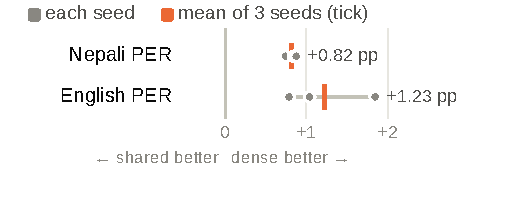
\includegraphics[width=\columnwidth]{figures/shared_vs_dense.pdf}
  \caption{\textbf{Shared-basis vs.\ dense at equal unique parameters (281K).} Difference in untouched-test PER (shared $-$ dense; $n=300$ NE + 300 EN) for three training seeds (gray) and their mean (orange). Dense is better on every seed in both languages.}
  \label{fig:shared}
\end{figure}

\paragraph{Multi-Seed Shared vs.\ Dense Trade-Off.}
At \texttt{seed=42}, \texttt{PAWP-300K Shared} achieved lower \texttt{val\_mel} (0.8768 vs.\ 0.8778), stronger \texttt{val\_energy} (1.50 vs.\ 1.60), and lower Code-Mix ASR WER (12.02\% vs.\ 18.09\%, $n=9$; not reproduced at $n=160$, see below). However, on the larger untouched $300+300$ \texttt{test.jsonl} PER benchmark, equal-unique-parameter \texttt{Dense-300K} outperformed \texttt{Shared} on \textbf{3 out of 3 independent seeds} (42, 101, 202) with zero overlap: Nepali PER averaged \textbf{5.53$\pm$0.08\%} vs.\ 6.35$\pm$0.11\% ($-0.82$\,pp; \texttt{seed=42} paired bootstrap 95\% CI $[+0.56, +1.41]$, $p<0.001$) and English PER averaged \textbf{5.34$\pm$0.28\%} vs.\ 6.57$\pm$0.47\% ($-1.23$\,pp; \texttt{seed=42} 95\% CI $[+1.44, +2.35]$, $p<0.001$), approaching \texttt{PAWP-1.5M v3} at 5.3$\times$ fewer parameters (Figure~\ref{fig:shared}). The confidence intervals capture utterance sampling within seed 42 only. Across seeds, the evidence is the sign of the difference (dense better in 6/6 seed$\times$language comparisons) and the non-overlapping seed ranges. Other metrics disagree: on the small held-out ASR set (seed 42), \texttt{Shared} has lower Nepali CER (5.93 vs.\ 6.59) and code-mix CER (5.01 vs.\ 9.01, $n=9$). Independent re-scoring resolves most of this disagreement. Under the independent phone recognizer, dense again wins all 6 seed$\times$language comparisons (EN 14.83$\pm$0.32\% vs.\ 16.28$\pm$1.14\%, NE 38.69$\pm$0.62\% vs.\ 40.51$\pm$0.42\%; paired $t$-test over the six pairs $p=0.010$, Wilcoxon $p=0.031$) and all 3 seeds on the code-mixed set (36.49\% vs.\ 39.47\% PER). Independent English ASR favours dense on all 3 seeds (WER 5.22\% vs.\ 8.13\%), while Nepali ASR is tied. The seed-42 code-mix advantage of \texttt{Shared} disappears on the 160-sentence set (18.78\% WER for both). The conclusion: at equal unique parameters, $K=2$ basis sharing gives no advantage, and dense is better on phone accuracy under both the training-time and an independent recognizer. Note that \texttt{Shared} materializes 17\% more compute parameters (328K vs.\ 281K), so a compute-matched comparison would favour dense further. Architectures: \texttt{Dense-300K} uses $d_{\text{model}}=58$, 3 encoder and 3 acoustic ConvNeXt blocks (FFN 116, kernels 5/7), rank-4 language residuals, and a 3-block decoder of width 88 (FFN 176) with a 257-bin iSTFT head ($n_{\text{fft}}=512$). \texttt{Shared} uses $d_{\text{model}}=64$ (FFN 128), $K=2$ shared bases with rank-8 per-layer residuals, 28-dim articulatory conditioning, and decoder width 96 (FFN 192). Both use duration/pitch/energy predictors of width 48/48/32.

\begin{table}[t]
\centering
\caption{\textbf{Independent re-scoring} (\texttt{EXP-018/019}). ASR: a second mixed-script recognizer not used for data filtering (held-out $n=30$ EN / 30 NE). PER: public \texttt{wav2vec2-xlsr-53-espeak-cv-ft} phone recognizer, both sides mapped to a shared 39-phone set (test $n=300$ EN / 300 NE). Mix: new 160-sentence code-mixed set (1,633 words), micro-averaged. 281K rows: mean$\pm$std over seeds 42/101/202.}
\label{tab:indep}
\footnotesize
\setlength{\tabcolsep}{2.5pt}
\resizebox{\columnwidth}{!}{%
\begin{tabular}{@{}lrrrrr@{}}
\toprule
 & EN & NE & EN & NE & Mix-160 \\
Model & CER & CER & PER & PER & WER / CER \\
\midrule
Human & 0.68 & 22.65 & 13.44 & 34.12 & --- \\
PAWP-1.5M & 2.35 & 19.46 & 15.14 & 38.10 & 18.13 / 8.80 \\
Shared-300K & 4.10{\scriptsize$\pm$0.52} & 21.07{\scriptsize$\pm$1.93} & 16.28{\scriptsize$\pm$1.14} & 40.51{\scriptsize$\pm$0.42} & 18.78 / 9.35 \\
Dense-300K & 2.44{\scriptsize$\pm$1.20} & 20.18{\scriptsize$\pm$0.78} & \textbf{14.83}{\scriptsize$\pm$0.32} & \textbf{38.69}{\scriptsize$\pm$0.62} & 18.78 / 9.00 \\
\bottomrule
\end{tabular}}
\end{table}

\paragraph{Latency and Zero-Shot Compression.}
On a 4-thread x86\_64 CPU (30 timed runs after 3 warm-up runs), the folded monolingual \texttt{PAWP-1.5M} ONNX graph computes its first 60\,ms audio chunk in 1.11\,ms p50 (1.52\,ms p99), i.e.\ 1.9\% of the chunk duration, and the frontend takes 0.16\,ms p50 per sentence. Over whole utterances, the measured real-time factor is 0.0058. Latency depends only on graph shape, so it was measured on the structural (untrained) graph; these are compute times measured after the utterance is encoded. In a later rerun of the trained graphs under the same protocol, the code-mixed graph (residuals unfolded, both languages active) took 1.24\,ms p50 per 60\,ms chunk vs.\ 0.96\,ms folded (+29\%; RTF 0.0055 vs.\ 0.0043). The 281K models took 0.70\,ms folded and 0.82--0.84\,ms unfolded (+17--19\%). Not yet measured: end-to-end time-to-first-audio with stateful streaming, and ARM/browser targets. Post-hoc one-shot SVD of the trained 1.5M model without recovery training (\texttt{EXP-010}; held-out ASR, $n=30/30/9$) raised English WER from 5.0\% to 14.3\% at 1.0M (uniform SVD) and to 66\% at 750K, and every method collapsed (WER $>100\%$) at 500K. The trained-from-scratch 281K models avoid this collapse, which suggests that compact end-to-end training is needed below $\sim$1M parameters.
